\subsection{Débit volumique}



\begin{definition}[Débit volumique]\label{def:Dv}
    Le débit volumique (noté \(D_{v}\)) est le volume du fluide \(V\) qui s'écoule par unité de temps à travers la section droite \(S\) de la conduite qui délimite le mouvement du fluide.
    \[
        D_{v} = \frac{dV}{dt} = \frac{V}{\Delta t} = S \cdot v 
    \] 
\end{definition}

\begin{explanation}

    Le volume du fluide s'écoulant pendant \(\Delta t\) est : 
    \[
        V = S \cdot L
    \]
    Où L est la distance parcourue par le fluide :
    \[
        L = v \cdot \Delta t
    \]
    On a par définition : \(D_{v} = \frac{V}{\Delta t}\)
    \[
        \implies D_{v} = \frac{S \cdot L}{\Delta} = S \cdot v \, \square  
    \]
\end{explanation}

\begin{figure}[!htb]
    \centering
    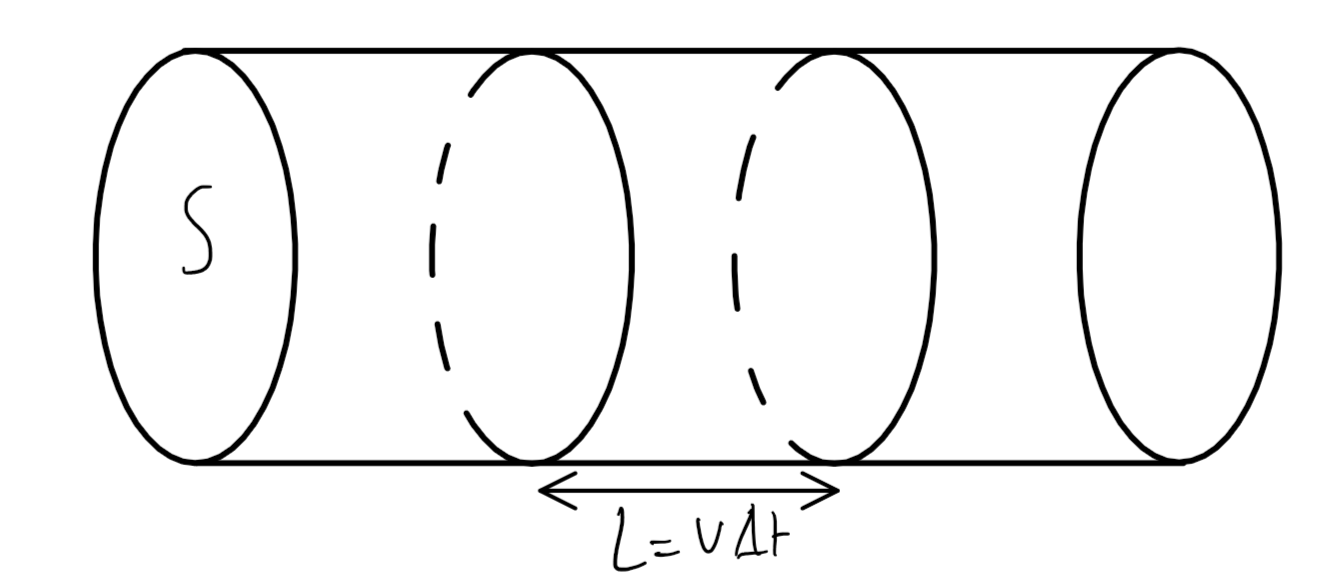
\includegraphics[width=0.8\textwidth]{SchemaDv.png}
    \caption{Schema du débit volumique dans une canalisation.}
    \label{fig:SchemaDv}
\end{figure}

\subsubsection{Conservation du débit volumique}

\begin{theorem}[Conservation du débit vomlumique]\label{thm:consdebitvol}
    Le débit volumique d'un fluide incompressible, parfait, en écoulement permanent est le même à travers toute section droite d'une canalisation.
\end{theorem}

\begin{corollary}[Conséquence]\label{col:propSV}
    On a : 
    \[
        v \cdot S = \text{ cste } \iff v \propto \frac{1}{S}
    \]
\end{corollary}

\section{Relation de Bernoulli}

\begin{definition}[Relation de Bernoulli]\label{def:relbern}
    La relation de Bernoulli traduit la conservation de l'énergie volumique d'un écoulement parfait, permanent et incompressible. C'est l'analogue de la conservation de l'énergie mécanique en mécanique du point.
\end{definition}

\begin{theorem}[Relation de Bernoulli]\label{thm:relbern}
    Si \(A\) et \(B\) appartiennent à la mmême ligne de courrant, alors, la densité énergétique \(\frac{E}{V}\) se conserve. (On prend l'axe \((Oz)\) orienté vers le haut)
    \[
        P_{A} + \frac{1}{2} \rho v_{A}^{2} + \rho g z_{A} = P_{B} + \frac{1}{2} \rho  v_{B}^{2} + \rho g z_{B}
    \] 
\end{theorem}

\begin{definition}[Energies du fluide]\label{def:efluide}
    On a :\\
    \begin{itemize}
        \item \(e_{c} = \frac{1}{2} \rho v^{2}\), la densité volumique d'énergie cinétique
        \item \(e_{z} = \rho g z\), la densité volumique d'énergie cinétique
        \item \(e_{p} = P\) la densité volumique du travail des forces pressantes. 
    \end{itemize}
\end{definition}

\begin{remark}[Equivalence avec la statique des fluides]
    Si le fluide est au repos (\(v = 0\) ), on retrouve la loi fondamentale de la statique des fluides.
\end{remark}